	\section{Redes inalámbricas}	
	Las redes inalámbricas son conjuntos de dispositivos informáticos comunicados entre sí  sin la necesidad de utilizar cables de ningún tipo. Las redes inalámbricas funcionan de manera similar a las redes cableadas, sin embargo, las redes inalámbricas deben convertir las señales de información en una forma adecuada para la transmisión a través del medio de aire. \\
	
	Las redes inalámbricas se pueden clasificar en cuatro grupos específicos según el área de aplicación y el alcance de la señal, como se muestra en la figura . Se llama alcance a la distancia máxima a la que pueden situarse las dos partes de la comunicación inalámbrica.
	
	\begin{figure}[htbp!]
		\centering
		\fbox{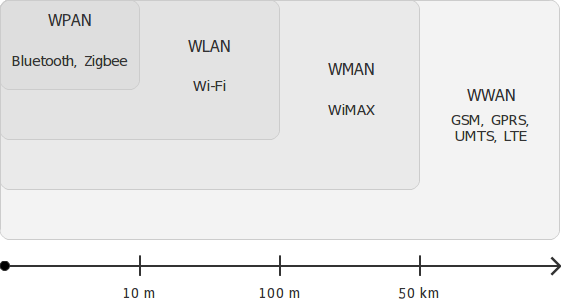
\includegraphics[width=0.8\textwidth]{MarcoTeorico/imagenes/redesInalambricas.png}}
		\caption{Tipos y alcance de redes inalámbricas.}
		\label{fig:tiposRedes}
	\end{figure}
	
	
	\subsection{Redes inalámbricas de área personal (Wireless Personal-Area Networks - WPAN)}
	Las redes inalámbricas de área personal permiten la comunicación en un rango de distancias muy corto, unos 10 metros, baja velocidad, menos de 1 Mbps y con necesidad de visión sin obstáculos.\\
	
	Una conexión realizada a través de una WPAN implica poca o ninguna infraestructura o conectividad directa fuera del enlace establecido. Esto permite soluciones pequeñas, eficientes en energía y de bajo coste que pueden ser implementadas en una amplia gama de dispositivos informáticos y de comunicación portátil y móvil, como ordenadores, PDA, impresoras, ratones, micrófonos, auriculares, etc.
	
	\subsection{Redes inalámbricas de área local (Wireless Local-Area Networks - WLAN)}
	Las redes inalámbricas de área local (WLAN) están diseñadas para proporcionar acceso inalámbrico en zonas con un rango típico de hasta 100 metros y son utilizadas dentro de un mismo edificio o grupo de edificios. Esto proporciona a los usuarios la capacidad de moverse dentro de un área de cobertura local y permanecer conectado a la red. 
	
	\subsection{Redes inalámbricas de área metropolitana (Wireless Metropolitan-Area Networks - WMAN)}
	Las redes inalámbricas de área metropolitana (WMAN) forman el tercer grupo de redes inalámbricas. Se llama redes inalámbricas de área metropolitana, WMAN (Wireless Metropolitan Area Networks), a aquellas redes que tienen una cobertura desde unos cientos de metros hasta varios kilómetros. El objetivo es poder cubrir el área de una ciudad o entorno metropolitano. 
	
	\subsection{nalámbricas de área amplia (Wireless Wide-Area Networks - WWAN)}
	Las redes inalámbricas de área amplia se extienden a miles de kilómetros y suelen utilizar frecuencias con licencia. Este tipo de redes se pueden mantener en grandes áreas, tales como ciudades o países, a través de los múltiples sistemas de satélites o ubicaciones con antena atendidos por un proveedor de servicios de Internet. Las WWAN permiten la interconexión de varios sistemas de comunicaciones ayudando a que ésta sea cada vez más globalizada.

	\section{Tecnologías inalámbricas}
	Existen muchas tecnologías diferentes que difieren en la frecuencia de transmisión utilizada, la velocidad y el alcance de sus transmisiones. Cada una de esas tecnologías posee diferentes características que la hacen adecuada para diferentes tipos de aplicaciones. Asimismo existen diferentes tecnologías que pueden ser implementadas al mismo tipo de aplicación. Algunas de las tecnologías más significativas y con mayor penetración en el mercado son las siguientes:
	
	\subsection{Bluetooth}
	Bluetooth es un enlace radio de corto alcance que aparece asociado a las Redes de Área Personal Inalámbricas (WPAN) y pertenece al estándar IEEE 802.15.1. Originalmente Bluetooth fue diseñado para comunicaciones omnidireccionales (punto a multipunto), de bajo consumo de energía, corto alcance y con dispositivos baratos, reemplazando el uso de cables y conectando los dispositivos a través de una conexión ad hoc por radio. \\
		
	Bluetooth trabaja en el rango de frecuencias de 2,402 GHz a 2,480 GHz (Banda ISM). Los terminales pueden estar en movimiento y no tener línea de vista entre sí; además, las velocidades de transmisión oscilan entre 720kbps y 1 Mbps. 
	
	\subsection{Zigbee}
	ZigBee está basado en el estándar IEEE 802.15.4 que fue desarrollado como un estándar global abierto para abordar las necesidades de fácil aplicación, alta fiabilidad, bajo costo, bajo consumo y bajas velocidades de transmisión de datos en redes de dispositivos inalámbricos.\\
		
	Zigbee fue creado con  con la finalidad de promover el desarrollo e implantación de una tecnología inalámbrica bidireccional de bajo coste vía radio, para usarla en dispositivos de domótica, automatización de edificios (inmótica), control industrial, periféricos de PC o sensores médicos.  Tiene velocidades comprendidas entre 20Kbps y 250Kbps y rangos de 10 m a 75 m y opera en las bandas sin licencia 2.4 GHz, 900 MHz y 868 MHz, lo suficiente para satisfacer las necesidades de un sensor y de automatización usando redes inalámbricas.
	
	\subsection{Familia IEEE 802.11 (WI-FI)}
	WI-FI es una de las tecnologías de comunicación inalámbrica mediante ondas más utilizada hoy en día basada en el estándar IEEE 802.11. 
	
	Los diversos tipos de Wi-Fi que existen  son los siguientes:
	\begin{itemize}
		\item Los estándares IEEE 802.11b, IEEE 802.11g e IEEE 802.11n disfrutan de una aceptación internacional debido a que la banda de 2,4 GHz está disponible casi universalmente, con una velocidad de hasta 11 Mbit/s, 54 Mbit/s y 300 Mbit/s, respectivamente.
		\item En la actualidad ya se maneja también el estándar IEEE 802.11ac, conocido como WIFI 5, que opera en la banda de 5 GHz y que disfruta de una operatividad con canales relativamente limpios. La banda de 5 GHz ha sido recientemente habilitada y, al no existir otras tecnologías (Bluetooth, microondas, ZigBee, WUSB) que la utilicen, se producen muy pocas interferencias. Su alcance es algo menor que el de los estándares que trabajan a 2,4 GHz (aproximadamente un 10 \%), debido a que la frecuencia es mayor (a mayor frecuencia, menor alcance).
	\end{itemize}

	
	\subsection{WiMAX}
	WiMAX es una tecnología de comunicaciones con arquitectura punto a multipunto orientada a proporcionar una alta velocidad de transmisión de datos a través de redes inalámbricas de área metropolitana.  Basada en el estándar IEEE 802.16, WiMAX proporciona accesos concurrentes en áreas de hasta 50 km de radio (WMAN) sin necesidad de visión directa con las estaciones base. Funciona por debajo de los 11 GHz y alcanza velocidades de hasta 70 Mbps.
	
	
	\subsection{GSM (Global System for Mobile Comunications)}
	GSM (Sistema Global para Comunicaciones Móviles) es una tecnología celular digital abierta que se utiliza para transmitir servicios móviles de voz y datos. GSM admite llamadas de voz y velocidades de transferencia de datos de hasta 9.6 kbps, junto con la transmisión de SMS (Servicio de Mensajes Cortos). \\

	GSM opera en bandas y espectros armonizados en la mayor parte del mundo, combinado con la capacidad de roaming internacional de GSM, permite a los viajeros acceder a los mismos servicios móviles en el hogar y en el extranjero. GSM permite llegar a individuos a través del mismo número de móvil en hasta 219 países. \\

	Las redes terrestres GSM ahora cubren más del 90\% de la población mundial. El servicio de roaming por satélite GSM también ha ampliado el acceso a servicios en áreas donde la cobertura terrestre no está disponible.

	